\externaldocument{Chapter4}
\externaldocument{Chapter3}

% Chapter 5

\chapter{Evaluation}
\label{Chapter5}
\lhead{Chapter 5. \emph{Evaluation}}

\label{sec:evaluation_plan}
In the first part of this chapter, we declare the most important
specifics about the process of the evaluation of the
implemented framework, the goal of which is to make
conclusions about whether or not we succeeded in achieving the
requirements we specified earlier. The evaluation will be done by
running a multi-step, fairly typical experiment both manually and with
the framework, so we can easily observe the differences.\\[0.3cm]
After specifying the process, we will go over the results of the
evaluation. First comes the part where we discuss the
results we got when running the experiment using the framework. Here,
we describe how the experiment was orchestrated: what processes were
used, how the test file's code looked like. Then we'll take a look at
how the experiment was run, what information was given to the user
during runtime and how much time it took. Then, we will go over the
steps of the experiment done by hand, starting from connecting to the
interactive job started by the framework previously, then proceeding
with the experiment, including a summary about what commands
were needed to be given and how much time the steps took. After that,
we'll compare the results concerning runtime and the produced traces,
including making observations about the visualizations. Then we
compare the two different methodologies used: the "old", manual method
with the usage of the newly implemented framework. By comparing the
methodologies, we try to draw a conclusion whether or not the usage of
the framework is more feasible in the long term than the manual
method. In the end, we take a look at the most important shortcomings
of the current version of the implementation, as well as ideas about
how we could overcome them.
\section{Methodology}
The experiment process used in the evaluation will consist of the same
steps as mentioned before in the Implementation chapter as an example
MPI experiment process (see \ref{fig:xpflow_example2}), used to collect
RL traces, which can be used for example for the development of
SMPI. The steps in the process are very generic though: we need to be
more precise about certain details of the experiment.
\subsection{Experiment specification}
\subsubsection{Prerequisites}
There are certain prerequisites that are assumed about the user's
environment when running the experiment.
\begin{itemize}
\item XPflow is needed to be present at the place of the execution of
the test. This can be the user's workstation or any feasible
environment.
\item In order to provide authentication without prompting for a
password, ssh-keys are needed to be configured correctly
  \begin{itemize}
  \item between the place of execution and the site,
  \item between the site and the nodes,
  \item and between the nodes (required by mpirun and trace\_gather).
  \end{itemize}
\item An image providing the feature described in \ref{sec:image}.
\item The benchmark to run is needed to be compiled and available in
  the path that we give the broadcast method of the benchmark.
\end{itemize}
If all these requirements are fulfilled, the experiment should run
without a problem.
\subsubsection{The benchmark}
There are a number of scalable benchmark suites developed for parallel
execution. For the purposes of evaluation, the NAS Parallel Benchmarks
suite\cite{jfy99} was chosen. Although it's been around for some time
and there are newer ones, the NAS suite consists of relatively simple
applications, with easy-to-understand behaviors. Since our goal right
now is not to solve complex problems but only to test our framework by
doing trace collection, the NAS benchmarks are perfect for our
purpose. We have to note though, that the framework is not
NAS-specific: any other MPI benchmark could be run with the
implementation.\\[0.3cm]
The benchmark chosen for doing the evaluation is
called \emph{lu.B.8}. The name consists of 3 parts. The first
part, \emph{lu} indicates what the experiment is about: as its name
suggests, the LU benchmark solves a system of equations represented
with a matrix, with the LU factorization method.\\[0.3cm]
The second part of the name, \emph{B} is an
indication about the complexity of the problem that the benchmark
solves. The NPB suite defines so-called "problem classes" for its
benchmarks. B is in the middle "standard" complexity category, being
more complex than the Small (S), the Workstation-size (W) and A, the
least complex "standard" problem size, but less complex than C and the
larger test problem sizes.\cite{d13}\\[0.3cm]
Finally, the number \emph{8} at the end of the benchmark's name
indicates how many parallel processes it is intended for to be solved:
for our purposes, we choose it to be 8, thus, we will allocate 8 nodes
for our experiment, each of them running 1 MPI process to solve the
problem.\\[0.3cm]
It's important to note that when doing the experiment, we assume that
the benchmark is already compiled, in a specified place in the user's
home folder, provided as a parameter to the broadcast method:
/home/dlehoczky/NPB3.3/NPB3.3-MPI/bin/lu.B.8. As a side note: for the
user \emph{dlehoczky}, the environment variable \emph{\$NPB\_DIR} is
set to /home/dlehoczky/NPB3.3/NPB3.3-MPI, thus it can be used as a
shortcut when accessing the benchmark.
\subsubsection{The environment}
For our experiment, we use the Grid'5000 testbed, discussed in greater
detail before, in \ref{sec:environment}. As we said before, there are
many different sites to choose from. During development,
many tests were needed to be done. Sometimes one or two sites were
undergoing maintenance or became unstable for various reasons. Towards
the end of the development process, the Lille site proved to be
reliable in terms of availability, this is why it was chosen as the
site to run our final tests on.
\subsubsection{The OS image}
\label{sec:image}
We use a customized image called
\emph{wheezy-x64-big-lehoo}. This image contains all the necessary
tools required to run the described process. These tools were
mentioned before, at \ref{sec:rl_traces}, when we talked about how to
collect RL traces, which this experiment is about. To reiterate, let's
sum up what our customized image contains in order to execute our
experiment process:
\begin{itemize}
\item OpenMPI 1.6.4;
\item the \emph{TAU}\cite{sm06} profiling tool;
\item the PAPI\cite{mbdh99}\cite{lmmsl01} interface to low-level
hardware counters (configured so it's linked to TAU, which uses it for
tracing);
\item the \emph{Program Database Toolkit (PDT)}\cite{lcmsmrr00} (also
configured to be linked to TAU);
\item the \emph{trace\_gather}\cite{ms11} MPI program;
\item \emph{Akypuera}\cite{s13}, a library to trace mpi applications
and generate paje trace files. (In our experiment, we only use
its \emph{tau2paje} trace converting script.)
\end{itemize}
\subsubsection{The experiment process}
\label{sec:experiment_process}
As mentioned before, the experiment process will consist of the same
steps as in the example discussed before
(see \ref{fig:xpflow_example2}).\\[0.3cm]
To prepare our experiment process, we start by
logging in to the frontend with our user. Then, we start an
interactive job, allocating the desired number (in our case, 8) of
nodes for a specified amount of time. We won't specify what nodes we
want, the system will decide which ones we get. Since there might be
performance disparities between two different sets of nodes, we make
sure to use the exact same set of nodes in the two experiments (the
one done manually and the one done with the framework). We do this by
running the experiment with the framework first, then connecting to
the job started by the framework and repeating the experiment
manually, starting from the deployment part. The node allocation is
not really an important part of the experiment, thus, it's not a
problem that it's omitted from the manual execution.\\[0.3cm]
As part of the process that we conduct in both experiments, first, we
deploy the previously mentioned (\ref{sec:image}) customized image on the
nodes. Then we broadcast the runnable (\emph{lu.A.8}) to every node's
/tmp directory. After that comes the step where we disable all but one
core on every node. The reasoning for this step has been discussed
previously (see \ref{sec:multiple_cores}). This concludes the
preparation stage.\\[0.3cm]
It is worth noting that, just like we did before at the
checkpointing example (see \ref{sec:checkpointing}), we put a
checkpoint right after deployment. This way, if we want to do another
experiment, we can reuse our already allocated and deployed
nodes. Since deployment is the longest process in the experiment, such
a checkpoint can come in really handy. As already discussed before, we
can modify anything in the experiment that comes after the checkpoint
- the execution will resume and execute the modified code.\\[0.3cm]
After the preparation stage comes the execution of the benchmark. We
use OpenMPI 1.6.4, installed on our image.\\[0.3cm]
After the running of the benchmark, comes the post-processing. If we
compiled our benchmark correctly with TAU, one trace file (.trc)
and one event file (.edf) is generated for each MPI process. The
traces are generated on the node of execution. This is why first,
we run the \emph{trace\_gather}\cite{ms11} script to collect the traces
and event files scattered across all the allocated nodes to the head
node. When we have all the files on our head node, we use
TAU's \emph{tau\_treemerge.pl}, which is a script that merges all our
trace files and event files into one trace and event file
respectively, also trying to account for any clock skew
(see \ref{sec:clock_synch}) between the trace files with
post-processing methods. Finally, when we have one merged trace and
one event file, we can convert our TAU trace to a format that is
compatible with the Pajé\cite{cob00} visualization tool. Visualizing
the traces makes it easier to analyze and compare. For the conversion,
we use Akypuera's\cite{s13} \emph{tau2paje} script.\\[0.3cm][0.5cm]

\section{Results}
In this part of the chapter, we go over how the experiments went by
observing their different stages. Then compare the results, the
two different methodologies and we discuss the shortcomings of the
framework.
\subsection{Experiment using the framework}
First, we discuss the experiment orchestrated with the test
framework. The test written with the framework consists of one single
file, containing 1 method (the main) and 11 function calls. We can
look at the code on figure \ref{fig:experiment_code}.\\[0.3cm]
The experiment itself can be divided into three main stages: the
preparation/configuration stage, the benchmark stage and the
post-processing stage.

\begin{figure}[htbp]
  \centering
    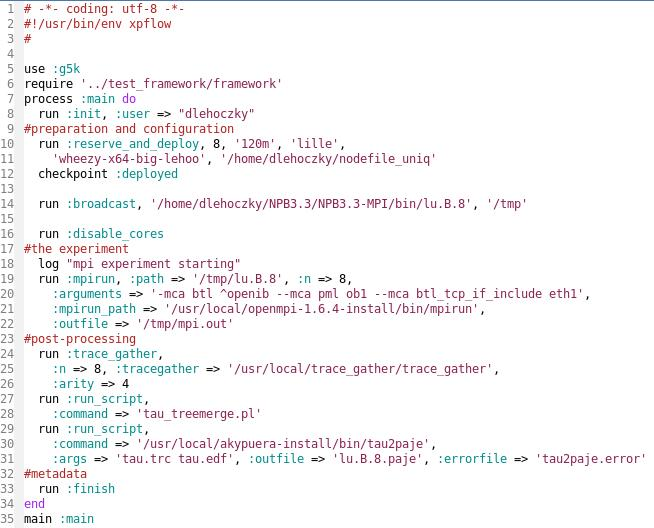
\includegraphics[scale=0.7]{./Figures/experiment_code.jpg}
    \rule{35em}{0.5pt}
  \caption[Experiment code]{The experiment, orchestrated with the test
    framework.}
  \label{fig:experiment_code}
\end{figure}

\subsubsection{Preparation}
\paragraph{Experiment initialization}
In the beginning of every experiment, the \emph{init} method has to be
called in order to configure certain variables with default values and
also to make configuration steps regarding metadata collection
(e.g. record the date of the experiment, the exact time of starting,
etc.). Also, here is where the user can set his/her username to log in
to the nodes. If not set, the username will default to root.
\paragraph{Reserve and deploy}
This is the part where the program starts a job by allocating 8 nodes
on the \emph{lille} site and deploying the image (given as a parameter
to the method) on them. We set the allocation time to 120 minutes (2
hours), which should give us plenty of time to execute the experiment
with both the framework and manually on the nodes.\\[0.3cm]
As part of the process, a so-called 'nodefile' is created, which
contains the names of all the nodes that we allocated. Originally, the
environment variable \emph{\$OAR\_FILE\_NODES} is set on the frontend
when logged in to an active job, with the value of the path to a file
containing the node names, each as many times as many cores they
have. During the experiment, we create a nodefile that only contains
each node once, so it can be used as a machinefile for certain
commands later. We specify a custom path to the nodefile with an
argument. If that argument is not set, our nodefile would be created
in the home folder anyway.\\[0.3cm]
Logs of the deployment process can be seen on
figure \ref{fig:fex_deployment}. As we can see, we allocate 8 nodes
for 2 hours of time. This means that after 2 hours, the job terminates
and we are disconnected from the nodes. In our case, the 2 hours
proved to be more than enough to conclude our tests. We can also
observe that while the node allocation only took a mere 22 seconds,
image deployment was taking much longer: it went on for about 8
minutes. In the end, we can see the "deployment complete" message,
notifying us that the image deployment process was successful and we
can now move on to the next stages of the experiment.

\begin{figure}[htbp]
  \centering
    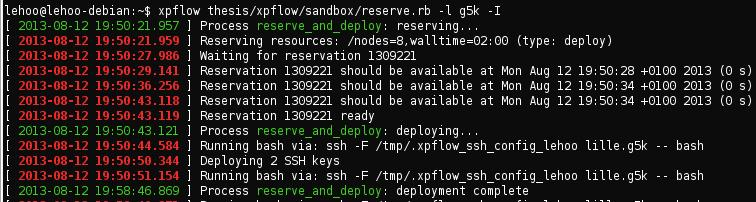
\includegraphics[scale=0.6]{./Figures/fex_deployment.jpg}
    \rule{35em}{0.5pt}
  \caption[Allocation and deployment]{Logs of the node allocation and
    image deployment process.}
  \label{fig:fex_deployment}
\end{figure}

\paragraph{Broadcasting the runnable}
The benchmark needs to be copied to every node to the path where the
execution will take place - otherwise MPI wouldn't be able to start
its processes on every node. The parameters here are pretty
straightforward - we give the method the path to the compiled
benchmark and the path to copy it to. The nodefile is not needed to be
given, since it's already been created and stored by the library
before.\\[0.3cm]
As it's a relatively fast and simple process, the framework doesn't
display any extra log messages to notify us of their success. Since
the benchmark was able to run, we can be sure that it succeded.
\paragraph{Disabling cores}
This is the method call that is responsible for disabling all but one
core on every node that takes part in the execution. We talked about
why this is necessary earlier, see \ref{sec:multiple_cores}. No
parameters are needed to be given here.\\[0.3cm]
This, like the broadcasting process, is a fast and relatively simple
process. Also, as previously mentioned, the fact whether or not the
cores were successfully disabled is checked in a loop, repeating the
disabling step until it's successful. Thus, we can be sure that this
step succeeded.
\subsubsection{Running the benchmark}
After all the configuration steps have been successfully done, it's
time for actually running the benchmark. As parameters, we first give
the \emph{mpirun} method call the path to the runnable (meaning, of
course, the path that we broadcasted the runnable to before, not its
original path) and the number of nodes, which, in our case, is 8. We
also specify the MPI runnable with its full path: this is to avoid
confusion about which version of MPI is actually running on the nodes,
ensuring that it's the version we deployed on the image (OpenMPI
1.6.4). If not given, it would be defaulted to simply 'mpirun'. We
specify the file to put the output of the benchmark to as well.\\[0.3cm]
We can put any extra arguments that we want to give to mpirun in the
"arguments" parameter. In this case, we use this parameter to specify
that our benchmark must not use Infiniband. This is needed because
SMPI is unable to simulate Infiniband connection, thus, a trace
acquired using it would show significantly better performance than the
simulated version.\\[0.3cm]
We can see logs produced when running the MPI benchmark, on
figure \ref{fig:fex_mpirun}. At the beginning of the method, the
framework logs the name of the designated head node, which is the node
the benchmark execution commands will be given and where the traces
will be gathered, merged and converted. This node, in our case, is the
node called \emph{chimint-6}.\\[0.3cm]
The execution time of the benchmark was 46.769 seconds. This result is
taken from the traces themselves, as we can see see below, at the
visualization of the traces.

\begin{figure}[htbp]
  \centering
    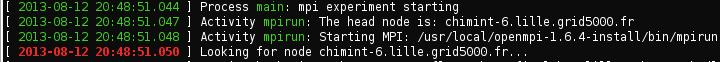
\includegraphics[scale=0.6]{./Figures/fex_mpirun.jpg}
    \rule{35em}{0.5pt}
  \caption[Benchmark execution]{Logs about the execution of the
    benchmark.}
  \label{fig:fex_mpirun}
\end{figure}

\subsubsection{Post-processing}
\paragraph{Gathering the traces}
As we mentioned before, in \ref{sec:experiment_process}, since we
compiled our benchmark with TAU, every MPI process produces
one trace (.trc) and one event (.evt) file. These traces are scattered
across the nodes. To gather them to one node, we use
the \emph{trace\_gather} MPI program. The method call with the same
name takes as parameter the number of nodes, the path to
the trace\_gather executable (the MPI executable is remembered
from the \emph{mpirun} call) and the arity parameter
(see \ref{sec:trace_gather}).
\paragraph{Merging the traces}
For running \emph{tau\_treemerge.pl}, we use the \emph{run\_script}
method of the framework, which is a generic method that executes the
command given as parameter on the head node. No other arguments are
needed in this case. Although we could specify files to put the output
and the error messages to, we don't really need that in this simple
case. The directory to merge the traces in defaults to "/tmp", so that
is not needed either. As we mentioned before, this script doesn't only
merge our traces, it also attempts at accounting for any clock skew.
\paragraph{Converting the traces}
As mentioned before, we use Akypuera's\cite{s13} \emph{tau2paje}
script to convert our traces to Pajé-visualizable format. For this, we
use the \emph{run\_script} method again, giving it the trace and event
files as arguments, as well as files to put the output and the error
messages to. Tau2paje generates error messages because of
synchronization problems (clock skew). As we described before
(see \ref{sec:clock_synch}), clock skew problems are really hard to
overcome. Although the merging script before tried to take care of the
problem, it can't eliminate it completely, but it does a well enough
job so this problem doesn't interfere with the conversion results in
any noticeable way.\\[0.3cm]
After the conversion is done, the visualizable trace file called
\emph{lu.B.8.paje} is available on the /tmp folder of the head
node. We can now copy it to our local machine and visualize the
result. (The results will be discussed below, after discussing the
manual experiment.)\\[0.3cm]
We can see logs about the post-processing part on
figure \ref{fig:fex_postprocessing}. We can see by the lines starting
with "Looking for the node chimint-6...", that the head node is the
same throughout the experiment, and the post-processing indeed happens
there. We can also observe that the post-processing takes about 30
seconds to complete.

\begin{figure}[htbp]
  \centering
    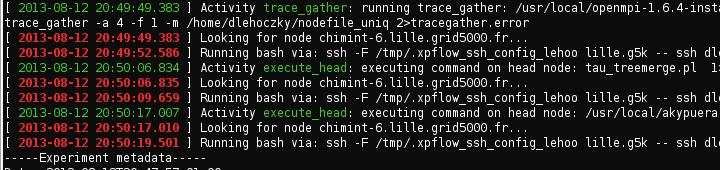
\includegraphics[scale=0.6]{./Figures/fex_postprocessing.jpg}
    \rule{35em}{0.5pt}
  \caption[Post-processing]{Logs about the post-processing part of the
    experiment.}
  \label{fig:fex_postprocessing}
\end{figure}

\subsubsection{Metadata}
In the end, we get some amount of metadata generated by the
experiment, summarizing some of its most important specifics, as it
can be seen on figure \ref{fig:fex_metadata}.\\[0.3cm]
It's worth pointing out that the framework keeps track of the time
before and after the checkpoint, which was placed at the
deployment. This way, we can easily distinguish between the time the
deployment took and the time the other parts of the experiment
took. It is obvious by looking at the times that the deployment
process is the longest part of the experiment.\\[0.3cm]
If we take a look at the nodes used, we can see that we used nodes
from 2 different clusters on the lille site: the
clusters \emph{chirloute} and \emph{chimint}.

\begin{figure}[htbp]
  \centering
    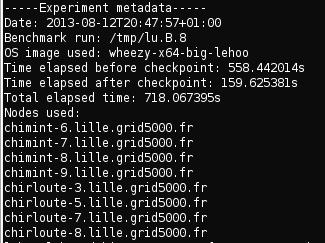
\includegraphics[scale=0.7]{./Figures/fex_metadata.jpg}
    \rule{35em}{0.5pt}
  \caption[Metadata]{Metadata produced by the framework about the
    experiment.}
  \label{fig:fex_metadata}
\end{figure}

\subsection{Experiment by hand}
Now, let's take a look at how the manual experiment went. As mentioned
before, the two experiments consist of the same exact steps. As
before, we divide the experiment into three main sections:
preparation stage, benchmark stage and post-processing stage.
\subsubsection{Preparation}
Table 5.1 is summarizing the results for the preparation and
configuration stage. The whole preparation stage took place on the
frontend of the site "lille", with the user "dlehoczky".

\renewcommand{\arraystretch}{1.5}
\begin{table}
\begin{center}
\begin{spacing}{1}
\caption{Preparation and configuration stage for the manual
experiment}
\begin{tabular}{| p{4cm} | p{8cm} | l |} \toprule
  \multicolumn{3}{ |c| }{\textbf{Preparation}} \\ \midrule
  \multicolumn{1}{ |c| }{\emph{Task}} & \multicolumn{1}{ |c|
  }{\emph{Command}} & \multicolumn{1}{ |c| }{\emph{Time
  (s)}}\\ \midrule
  Reserving nodes & Omitted - joined the existing job,
  using the already allocated nodes & - \\
  Deployment & \texttt{\small kadeploy3 -f \$OAR\_FILE\_NODES -e
  wheezy-x64-big-lehoo} & 453.343 \\
  Create a nodefile containing all the node names only once
  & \texttt{\small cat   \$OAR\_FILE\_NODES | uniq > \textasciitilde
  /nodefile\_uniq} & 0.004 \\
  Broadcast of runnable & \texttt{\small taktuk -l dlehoczky -f
  \textasciitilde /nodefile\_uniq broadcast put
  { \$NPB\_DIR/bin/lu.B.8 } { /tmp }} & 0.389 \\
  Disabling cores & \texttt{\small taktuk -l root -f /home/dlehoczky/nodefile\_uniq
  broadcast exec [ 'for i in /sys/devices/system/cpu/ cpu[1-9]*/online;
    do echo 0 > "\${i}" ; done' ]} & 1.974 \\
  \emph{Optional}: Check if the cores have been disabled accordingly
  & \texttt{\small taktuk -f \textasciitilde /nodefile\_uniq broadcast
  exec [ 'cat /proc/cpuinfo' ] | grep process | awk '{if(\$9>0)
  print \$1}' | uniq | awk -F".fr-" '{print \$1".fr"}'} &
  1.319 \\ \midrule
\end{tabular}
\end{spacing}
\end{center}
\end{table}

As a side note: when doing the core disabling with the framework, the
program repeats the disabling step until it confirms it to be
successful, with the step marked as "Optional" here. In the step where
we check if the cores are disabled, every node name is displayed that
has more than 1 core running. The disabling step needs to be repeated
until we don't see any node names when running that command. When
running the test, the disabling step was successful the first time,
thus there was no need to repeat that step.
\subsubsection{Running the benchmark}
Table 5.2 is about the command that was given to run the
benchmark (which is exactly the same as it was for the framework), as
well as its runtime. The benchmark had to be run from the directory
the benchmark was broadcasted to (/tmp in our case), on the designated
head node (which was, in our case, \emph{chimint-6}, the same as it
was for the framework.

\begin{table}
\begin{center}
\begin{spacing}{1}
\caption{Benchmark execution stage for the manual experiment}
\begin{tabular}{| p{4cm} | p{8cm} | l |} \toprule
  \multicolumn{3}{ |c| }{\textbf{Running the benchmark}} \\ \midrule
  \multicolumn{1}{ |c| }{\emph{Task}} & \multicolumn{1}{ |c|
  }{\emph{Command}} &   \multicolumn{1}{ |c| }{\emph{Time
  (s)}}\\ \midrule
  Running the benchmark
  & \texttt{\small{/usr/local/openmpi-1.6.4-install
  /bin/mpirun -mca
  btl \textasciicircum openib --mca pml ob1 -machinefile
  \textasciitilde /nodefile\_uniq -np 8 /tmp/lu.B.8 1>/tmp/mpi.out}}
  & 46.559 \\ \midrule
\end{tabular}
\end{spacing}
\end{center}
\end{table}

\subsubsection{Post-processing}
After executing the benchmark, the produced traces are sitting on
their respective nodes. In table 5.3, we summarize how the post-processing of
the files went. This stage of the experiment, as it was for the
benchmark, was executed on the head node, from the /tmp directory.

\begin{table}
\begin{center}
\begin{spacing}{1}
\caption{Post-processing stage for the manual experiment}
\begin{tabular}{| p{4cm} | p{8cm} | l |} \toprule
  \multicolumn{3}{ |c| }{\textbf{Post-processing}} \\ \midrule
  \multicolumn{1}{ |c| }{\emph{Task}} & \multicolumn{1}{ |c|
  }{\emph{Command}} & \multicolumn{1}{ |c| }{\emph{Time
  (s)}}\\ \midrule
  Gathering the traces & \texttt{\small/usr/local/bin/mpirun
  -machinefile \textasciitilde /nodefile\_uniq -np 8
  /usr/local/trace\_gather/trace\_gather -f 1 -a 4 -m \textasciitilde
  /nodefile\_uniq} & 8.152 \\
  Merging the traces & \texttt{\small tau\_treemerge.pl} & 3.967 \\
  Converting the trace to Pajé-compatible format & \texttt{\small
  /usr/local/akypuera-install/bin/tau2paje tau.trc tau.edf
  1>lu.B.8.paje 2>tau2paje.error} & 10.532 \\ \midrule
\end{tabular}
\end{spacing}
\end{center}
\end{table}

As mentioned previously at the end of the experiment with the
framework: after the conversion process, the file \emph{lu.B.8.paje}
is available on the head node, in its /tmp folder. Now, we can use
scp, rcp or some other program to download it to our local machine
from the remote node.
\section{Comparison}
\subsection{Comparison of results}
First, let's take a look at how much time the experiments took. Below
is a table summarizing the elapsed time for both experiments.

\definecolor{light-gray}{gray}{0.90}
\begin{center}
\begin{spacing}{1}
\begin{table}
\caption{Experiments - elapsed time}
\begin{tabular}{| c | c | c |} \toprule
  \multicolumn{1}{ |c|
  }{\multirow{2}{*}{\Large \textbf{\emph{Stage}}}} & \multicolumn{2}{
  |c| }{\textbf{\emph{Time (s)}}} \\ \cmidrule{2-3}
  & \multicolumn{1}{ |c| }{\emph{Experiment
  with the framework}} & \multicolumn{1}{ |c| }{\emph{Manual
  experiment}}\\ \midrule
  Preparation & 558.442 & 457.03 \\
  Running the benchmark & 46.767 & 46.559 \\
  Post-processing & 30.118 & 22.651 \\ \midrule
  The whole experiment & 635.327 & 526.24 \\ \midrule
\end{tabular}
\end{table}
\end{spacing}
\end{center}

We can see that although the preparation steps and the post-processing
took more time with the framework, the actual running of the benchmark
took the same amount of time. The time difference in the preparation
is most likely caused by disparity availability of resources to do the
deployment, and the fact that in the second case, we didn't have to do
the node allocation. Another likely reason, that applies to the
post-processing part as well, is simply the fact that we're doing
real-life traces and as such, running time can be different, as well
as results can differ. This is especially true for distributed
systems, where the exact sequence of messages sent is never the same,
in our case, between 8 nodes.
Now, let's take a look at the generated traces. We can see the traces
for both experiments, visualized with Vite, a Pajé visualization tool
on figures \ref{fig:fex_traces} and \ref{fig:mex_traces}.

\begin{figure}[htbp]
  \centering
    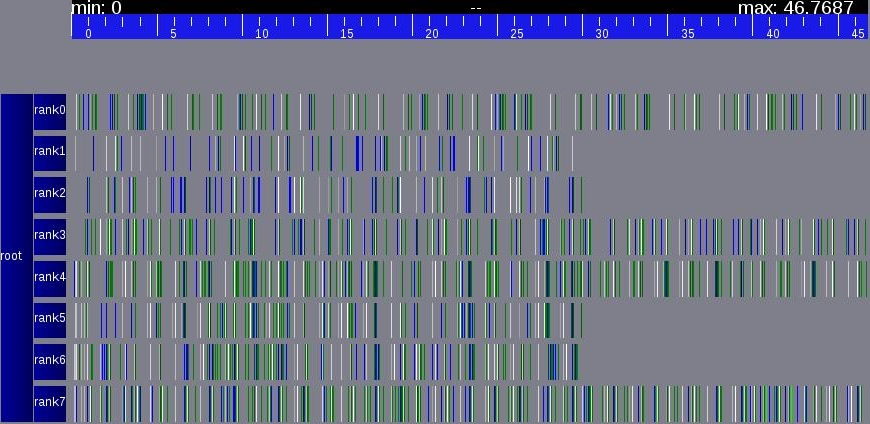
\includegraphics[scale=0.7]{./Figures/lu_B_8_framework.jpg}
    \rule{35em}{0.5pt}
  \caption[Traces from the experiment run with the framework]{Traces
    from the run with the framework, visualized with Vite.}
  \label{fig:fex_traces}
\end{figure}

\begin{figure}[htbp]
  \centering
    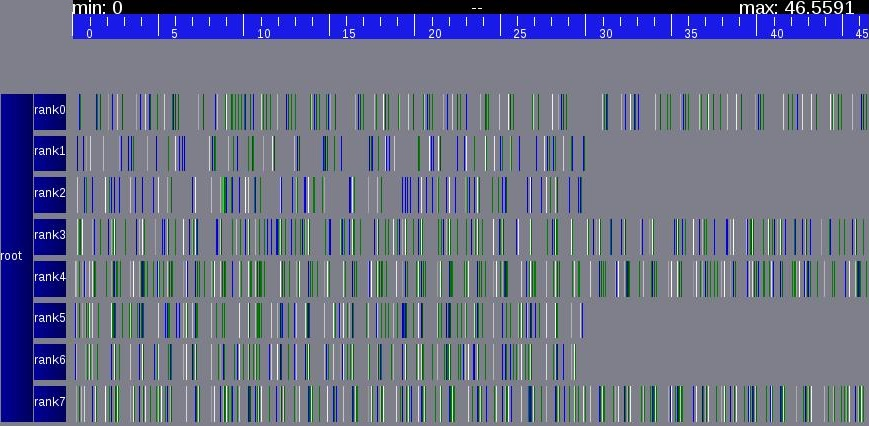
\includegraphics[scale=0.7]{./Figures/lu_B_8_manual1.jpg}
    \rule{35em}{0.5pt}
  \caption[Traces from the experiment run manually]{Traces from the
    run manually, visualized with Vite.}
  \label{fig:mex_traces}
\end{figure}

At first glance, it is apparent that the visualizations are made up of
differently colored lines. These lines represent the different MPI
operations. The X axis is the time. We can see that it starts from
zero, and ends at the time period equal to the benchmark's
runtime. The Y axis represents the different MPI processes, identified
by their rank - we can see the different ranks on the left side. Each
rank forms a horizontal "stripe" of its own, with the MPI operations
belonging to it inside that stripe. As for the MPI operations
themselves: the send operations (MPI\_Send()) are blue, the receive
operations (MPI\_recv()) are green, and the wait operations
(MPI\_Wait()) are white in color.\\[0.3cm]
If we observe the two trace visualizations, it is apparent that there
are obvious differences between them - the MPI operations didn't
happen at the same time. Sometimes, one of the experiments executed
more operations than the other in the same time interval and vice
versa. But if we disregard the smaller details, it's also visible that
the two visualizations are indeed very similar to each other: in both
cases, after roughly 29 seconds of execution time, only the processes
with the ranks 0, 3, 4 and 7 continue to execute operations. Due to
the nature of the benchmark, only 4 processes are used from that time.
\subsection{Comparison of methodology}
In the section before, we made the observation that the two methods -
the manual and the one with the framework - produce similar
results. Now the question remains: how do the two methods fare against
each other in other terms, not directly tied to the correctness of the
test results, but rather tied to the methodology.
\paragraph{Reliability}
The problem with the manual method in this regard is that it's
repetitive work and all the commands have to be given individually,
with certain modifications here and there. An obvious advantage for
the framework in this regard is that if it was working once, it will
be working again if we don't modify anything. If something is wrong,
but wasn't wrong the last time, we can be sure that the environment is
at fault - with the manual method, we can never be sure in that, as
there is always the chance that we mistyped something or left a step
out of the process this time.
\paragraph{Reusability}
This is strongly tied to the previous paragraph: after we write a
test's code with the framework, we can save that code and execute it
as many times as we want. We can't do that with the manual steps,
where we have to give the same commands individually again and
again. Bash history and scripts can help our work, but the more
experiments we do, the harder it's going to be to organize
them. Experiments written using the framework can be also organized
into higher-level workflows, providing the potential to run as many
tests as we need, one after the other. The only thing we need to pay
attention to is to correctly store our traces: making sure to copy
them to a more permanent location, each given a unique name, as well
as providing enough space to store all of them - trace files get
proportionally larger, the more complex and more large scale our
problems are.
\paragraph{User interaction}
Although this might seem to be a minor concern, in the long run, this
advantage of the framework can prove to be most valuable: when running
experiments manually, the user needs to pay attention to when the
command he/she gave finishes executing, then input the other command,
right until the end of the experiment. While when using the framework,
we only need to start the execution, which will then, as we saw,
automatically executes the consecutive steps, freeing up the user to
do other things while it's running. We can even set up our experiment
so it copies the traces to its permanent location, so we needn't to
worry about that either. As mentioned before, we can also tie together
multiple experiments into a single workflow easily. And this is
exactly what our main goal was at the beginning: to make the
researchers' lives easier.
\paragraph{Testing speed}
Again, this is closely tied to other viewpoints already mentioned. Due
to the fact that no user interaction is required, as well as the fact
that we have the possibility to run as many benchmarks in a single
workflow as we want, we can potentially run proportionally more
benchmarks, thus producing proportionally more traces and results in
other forms, which, as mentioned before, is much needed in our case
for validating SMPI.\\[0.5cm]
In this chapter, we first went over the specifics of the evaluation of
our implementation. We talked about the chosen benchmark to
gather traces from. We also discussed what the chosen
environment is going to be (Grid'5000) and what operating system image
we are going to deploy on our nodes before running the benchmarks on
them. After that, we went over the experiment process: the RL trace
collection for a given benchmark. We mentioned that our experiment
process will be done using two methods: we run it with and without the
framework to demonstrate how the two methods differ from each
other, in order to make a conclusion about whether or not it's worth
to use our implementation. Then we went on to discuss the process
itself: the preparation steps, the running of the benchmark and the
post-processing part.\\[0.3cm]
The section after that was about the results of running the
experiment with the two methods. We first went over the experiment
orchestrated with the framework in detail: we observed how the code
looked like, then went on to discuss the different stages: the
preparation and configuration stage, the running of the benchmark and
the post-processing stage, then taking a look at the metadata
produced. After that came the manual experiment. Similarly, we went
through the stages, this time summarizing what the commands and the
elapsed time were for each step. Then we went on to compare the two
methods: first, we compared the results, taking into account both the
elapsed time and the collected traces. We made observations about the
visualizations, concluding that the results were very similar,
although there are differences in details such as the sequence of the
MPI operations or their timings. The next part of this chapter was
about comparing the two methods by aspects not directly related to the
numerical results. These included reliability, reproducibility, user
interaction and testing speed. We concluded that indeed the
implemented framework possesses those advantages over the manual
method that we were aiming for. In the end, we went over some of the
current shortcomings of the implementation, along with some ideas
about what could be done to overcome them.
